\documentclass{article}
\usepackage{amssymb}
\usepackage{amsfonts}
\usepackage{amsmath}
\usepackage{cancel}
\usepackage{graphicx}
\graphicspath{ {./assets/} }
\author{Enlai Li}
\title{MATH240 -- Lecture 2}
\date{January 6, 2023}
\begin{document}
\maketitle
\section{Set algebra}
When are sets equal? For instance:
\begin{align*}
    A & = \{x \in \mathbb{Z} \ | \ x=2k-1 \text{ for some } k \in \mathbb{Z}\} \\
    B & = \{x \in \mathbb{Z} \ | \ x=2n+1 \text{ for some } n \in \mathbb{Z}\}
\end{align*}
We need to prove:
\begin{enumerate}
    \item $A \in B$
    \item $B \in A$
\end{enumerate}
1. NTS (need to show): if $x \in A$ then $x \in B$
\begin{gather*}
    \text{Assume } x \in A \text{ so } x = 2k-1 \text{ for some }k\in \mathbb{Z}
    = 2k-2+2-1
    =2(k-1)+1  \\
    \text{With }n=k-1 \text{ we have }x=2n+1 \\ \text{ therefore } A=B
\end{gather*}
2. $x \in B \Rightarrow x\in A$
Let $x=2n+1 \text{ where } n\in \mathbb{Z}$, then
\begin{align*}
    x & =2n+2-2+1 \\
      & =2(n+1)-1
\end{align*}
If $k=n+1$ then $x=2k-1 \Rightarrow x\in A$

\section{Set operations}

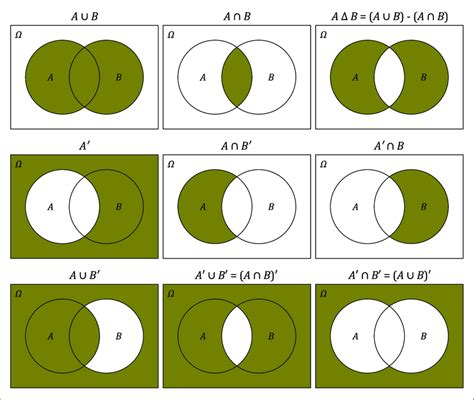
\includegraphics[width=\textwidth]{l1_venn_ab}
$U =$ The universe of objects
\begin{itemize}
    \item Union
          \[
              A \cup B =\{x\in U \ | \ x \in A \text{ or } x \in B\}
          \]
    \item Intersection
          \[
              A \cap B = \{x \in U \ | \ x \in A \text{ and } x \in B\}
          \]
    \item Difference
          \[
              A \backslash B = A-B = \{x \in A \ | \ x \notin B\}
          \]
    \item Complement \[
              \overline{A} = A' = \{x \in U \ | \ x \notin A\} = U \backslash A
          \]
\end{itemize}
\end{document}